\documentclass{standalone}
\usepackage{pgfplots}
\usepackage{lmodern}
\pgfplotsset{compat=1.17}

\begin{document}

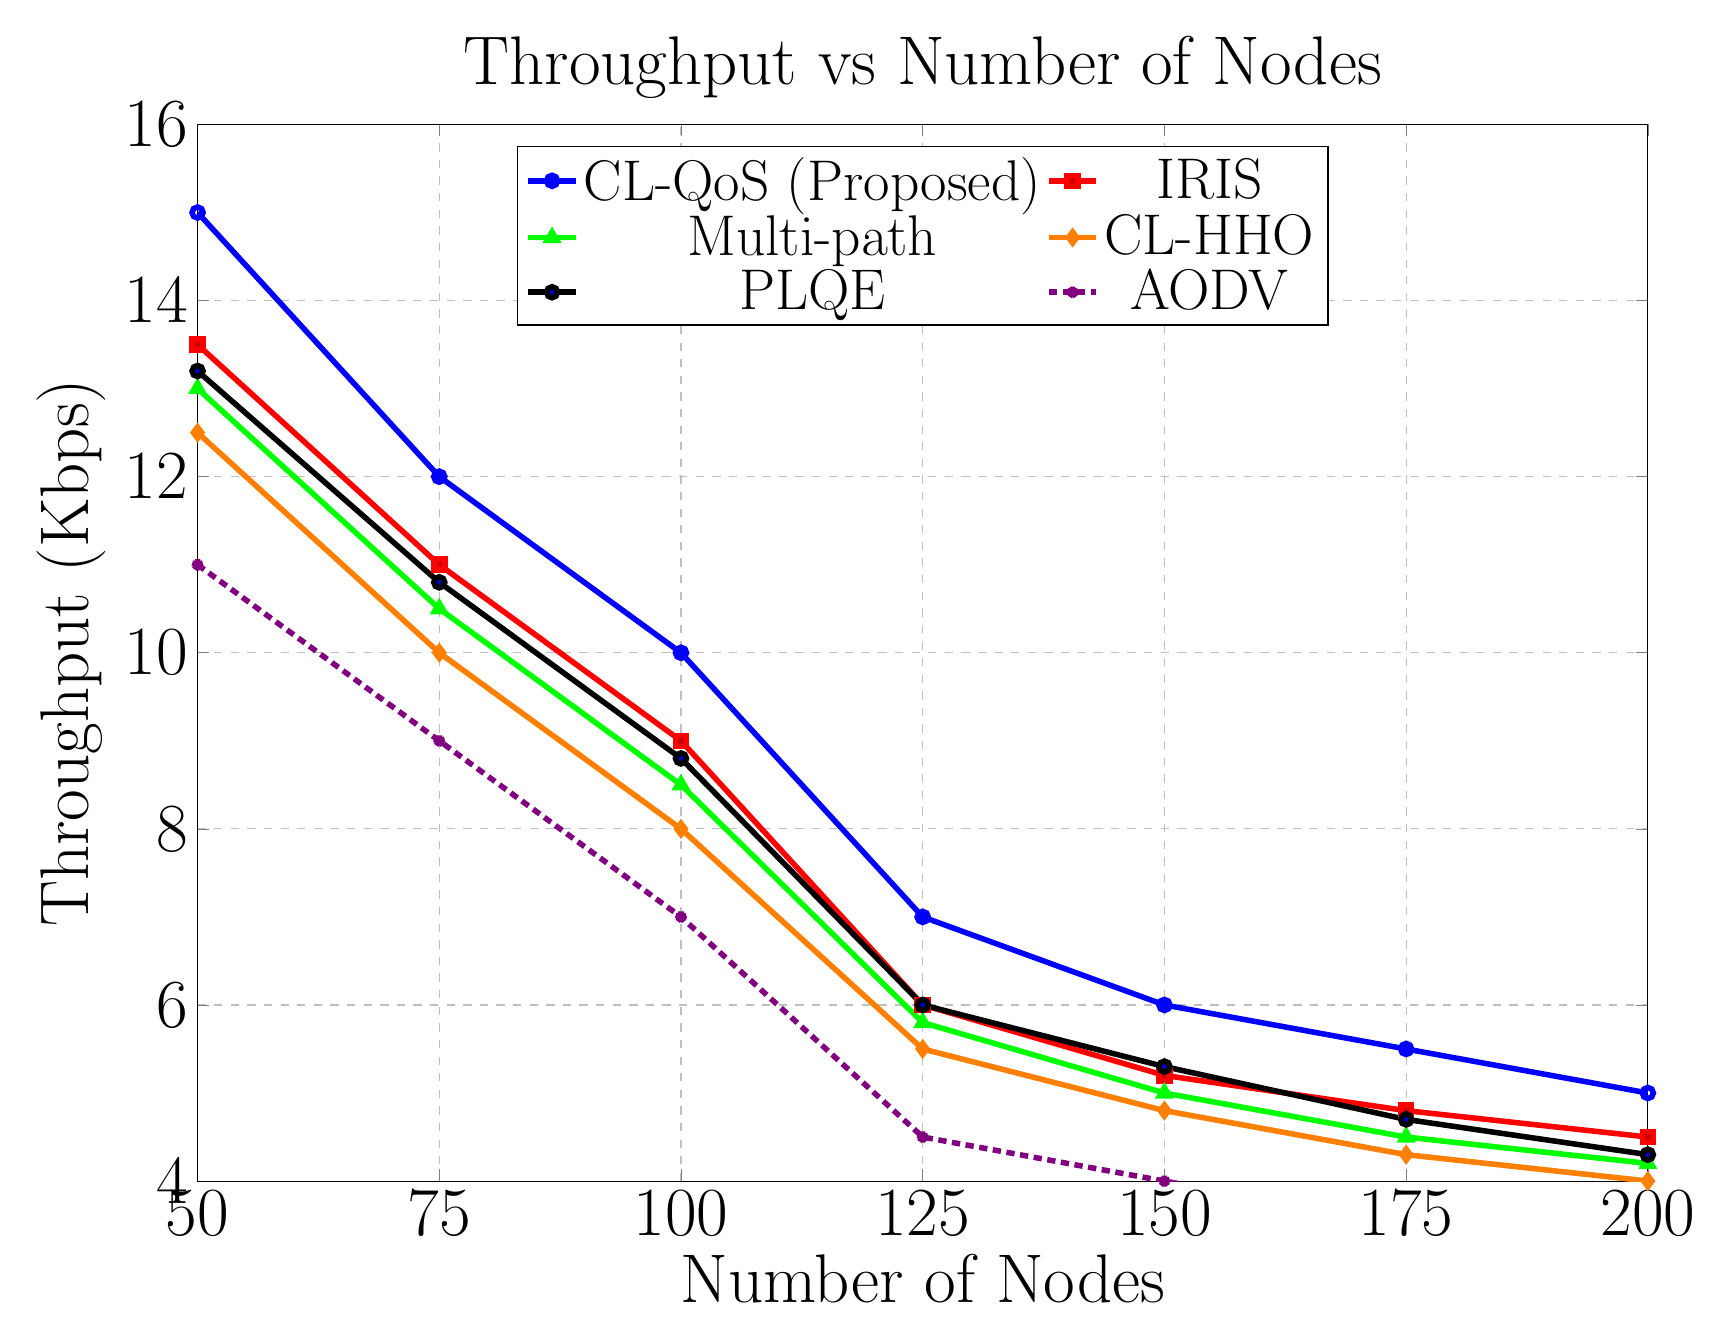
\begin{tikzpicture}
\begin{axis}[
    width=20cm,
    height=15cm,
    tick label style={font=\fontsize{24}{28}\selectfont},
    label style={font=\fontsize{24}{28}\selectfont},
    title style={font=\fontsize{24}{28}\selectfont},
    title={Throughput vs Number of Nodes},
    xlabel={Number of Nodes},
    ylabel={Throughput (Kbps)},
    xmin=50, xmax=200,
    ymin=4, ymax=16,
    xtick={50,75,100,125,150,175,200},
    ytick={4,6,8,10,12,14,16},
    legend columns=2,
    legend style={
        font=\fontsize{22}{26}\selectfont,
        at={(0.5,0.98)},
        anchor=north,
        draw=black,
        fill=white
    },
    ymajorgrids=true,
    xmajorgrids=true,
    grid style=dashed
]

% CL-QoS (Proposed)
\addplot+[mark=o,color=blue,line width=2pt] coordinates {
    (50,15)(75,12)(100,10)(125,7)(150,6)(175,5.5)(200,5)
};

% IRIS
\addplot+[mark=square*,color=red,line width=2pt] coordinates {
    (50,13.5)(75,11)(100,9)(125,6)(150,5.2)(175,4.8)(200,4.5)
};

% Multi-path
\addplot+[mark=triangle*,color=green,line width=2pt] coordinates {
    (50,13)(75,10.5)(100,8.5)(125,5.8)(150,5)(175,4.5)(200,4.2)
};

% CL-HHO
\addplot+[mark=diamond*,color=orange,line width=2pt] coordinates {
    (50,12.5)(75,10)(100,8)(125,5.5)(150,4.8)(175,4.3)(200,4)
};

% PLQE
\addplot+[mark=*,color=black,line width=2pt] coordinates {
    (50,13.2)(75,10.8)(100,8.8)(125,6)(150,5.3)(175,4.7)(200,4.3)
};

% AODV
\addplot+[mark=star,color=violet,line width=2pt] coordinates {
    (50,11)(75,9)(100,7)(125,4.5)(150,4)(175,3.5)(200,3)
};

\legend{CL-QoS (Proposed), IRIS, Multi-path, CL-HHO, PLQE, AODV}

\end{axis}
\end{tikzpicture}

\end{document}